\documentclass[a4paper,12pt,bibliography=totoc, listof=totoc,titlepage]{scrartcl}
\usepackage[ngerman]{babel}
\usepackage[utf8]{inputenc}
\usepackage[left=3cm,right=2.5cm,top=2.5cm,bottom=2.5cm]{geometry}
\usepackage[onehalfspacing]{setspace}
\renewcommand{\arraystretch}{1.5}
\usepackage{graphicx}
\usepackage{color}
\usepackage[dvipsnames,usenames,dvipsnames,table,xcdraw]{xcolor}
\usepackage[toc,page]{appendix}
\usepackage[printonlyused]{acronym}
%\usepackage[scaled]{berasans}
%\renewcommand*\familydefault{\sfdefault}  %% Only if the base font of the document is to be sans serif
%\usepackage[T1]{fontenc}

% Absatz-Einstellungen
\setlength{\parindent}{0pt} % Einrücken
\setlength{\parskip}{6pt}  % Horizontaler Abstand

\usepackage{subcaption}
\usepackage{graphicx} % omit 'demo' for real document
  
\usepackage[hyphens]{url}
\usepackage[hidelinks]{hyperref}
\setlength {\marginparwidth }{2cm}
\usepackage{todonotes}
\usepackage{amsmath}
\usepackage{cancel}

% Kommentare mit \begin{comment}
\usepackage{verbatim}

\usepackage{multirow}

\newcommand*\justify{%
  \fontdimen2\font=0.4em% interword space
  \fontdimen3\font=0.2em% interword stretch
  \fontdimen4\font=0.1em% interword shrink
  \fontdimen7\font=0.1em% extra space
  \hyphenchar\font=`\-% allowing hyphenation
}

\newcommand{\code}[1]{\texttt{\justify{#1}}}
%\usepackage{tocloft}

%Boxfehler
\hbadness=1000000

% Hurenkinder und Schusterjungen verhindern
\clubpenalties 3 10000 10000 1000
\widowpenalties 3 10000 10000 1000
\displaywidowpenalty=10000

% Listings
\usepackage{listings}
\lstset{
   breaklines=true,
   captionpos=t,
   basicstyle=\scriptsize\ttfamily,
   keywordstyle=\bfseries\ttfamily\color{orange},
   stringstyle=\color{green}\ttfamily,
   commentstyle=\color{gray}\ttfamily,
   emph={square}, 
   emphstyle=\color{blue}\texttt,
   emph={[2]root,base},
   emphstyle={[2]\color{yac}\texttt},
   showstringspaces=false,
   flexiblecolumns=false,
   tabsize=2,
   numbers=left,
   numberstyle=\tiny,
   numberblanklines=false,
   stepnumber=1,
   numbersep=10pt,
   xleftmargin=15pt
 }

% Zitierstil
%\usepackage[style=authoryear,citestyle=authoryear,natbib=true]{biblatex}
%\bibliography{Thesis.bib}
\usepackage[round]{natbib}
\bibliographystyle{hcu}

\begin{document}
\pagenumbering{Roman}
\begin{titlepage}
\begin{center}
\renewcommand{\arraystretch}{0.7}
\begin{tabular}{lr}
\begin{tabular}{l}

\includegraphics[width=0.35\textwidth]{img/hculogo_grau.png}
\end{tabular} \hspace{1.2cm} &
\begin{tabular}{r}
Universität für \\Baukunst und Metropolenentwicklung\\
Henning-Voscherau-Platz 1\\
20457 Hamburg\\
\end{tabular}
\end{tabular}\\\vspace{5cm}
\doublespacing 
{\huge\bfseries UAV-Flugplaner}\vspace{0.5cm}\\

{\large\bfseries Geodäsie und Geoinformatik\\WebGIS\\Sommersemester 2022}\vspace{2cm}\\
{\large Florian Timm (6028121)}

% hspace und vspace bedeutet horizontaler bzw. vertikaler Abstand
\vspace{7cm}
Abgabedatum: 30. September 2022
\end{center}
\setcounter{page}{0} % Seitenzahl wird auf 0 gesetzt 
\end{titlepage}


% Mehrere gleichzeitig zitieren
\providecommand{\citeTwo}[4]{\citep[{\citealp[#1]{#2};}][#3]{#4}} 
\providecommand{\citeThree}[6]{\citep[{\citealp[#1]{#2}; \citealp[#3]{#4};}][#5]{#6}} 
\providecommand{\citeFour}[8]{\citep[{\citealp[#1]{#2}; \citealp[#3]{#4}; \citealp[#5]{#6};}][#7]{#8}}

\newpage

\tableofcontents
\newpage

\pagenumbering{arabic}
\setcounter{page}{1} 

\section{Einleitungen und Funktionen}
Der UAV-Flugplaner dient der Planung von Befliegungen mittels UAV wie Multikoptern zur Erzeugung von Orthophotos und digitalen Geländemodellen. Er ermöglicht die Planung der einzelnen Aufnahmepunkten sowie die Abschätzung der Bilderanzahl, Fluglänge und -dauer. Außerdem sind Flugverbote hinterlegt, so dass eine grobe Planung der benötigten Genehmigungen ermöglicht wird.

\section{Installation}
Technisch basiert der Flugplaner auf Typescript, einem Javascript-Aufsatz (weitere Details in \autoref{technische_information}). Zur Ausführung wird Node.js benötigt. Weitere Abhängigkeiten werden automatisch nachgeladen.

Der Download kann von GitHub erfolgen
\begin{lstlisting}[language=bash]
git clone http://github.com/FlorianTimm/uavplanning.git
cd uavplaning
\end{lstlisting}

Die Installation der Abhängigkeiten des Backend und der Start erfolgt mit
\begin{lstlisting}[language=bash]
cd server
npm install
npm run serve
\end{lstlisting}

Anschließend können die Abhängigeiten des Frontend installiert und gestartet werden:
\begin{lstlisting}[language=bash]
npm install
npm run start
\end{lstlisting}

Sofern keine Ports bereits vorher belegt waren, ist der Planer dann unter \url{http://localhost:9000/} erreichbar.

\section{Bedienung}

Die Bedienung erfolgt als Webanwendung im Browser. Der Startbildschirm ist in \autoref{img:screenshot} zu sehen.

\begin{figure} % setzt die Abbildung an genau diese Stelle, sonst landet sich oben auf der Seite
 \centering
 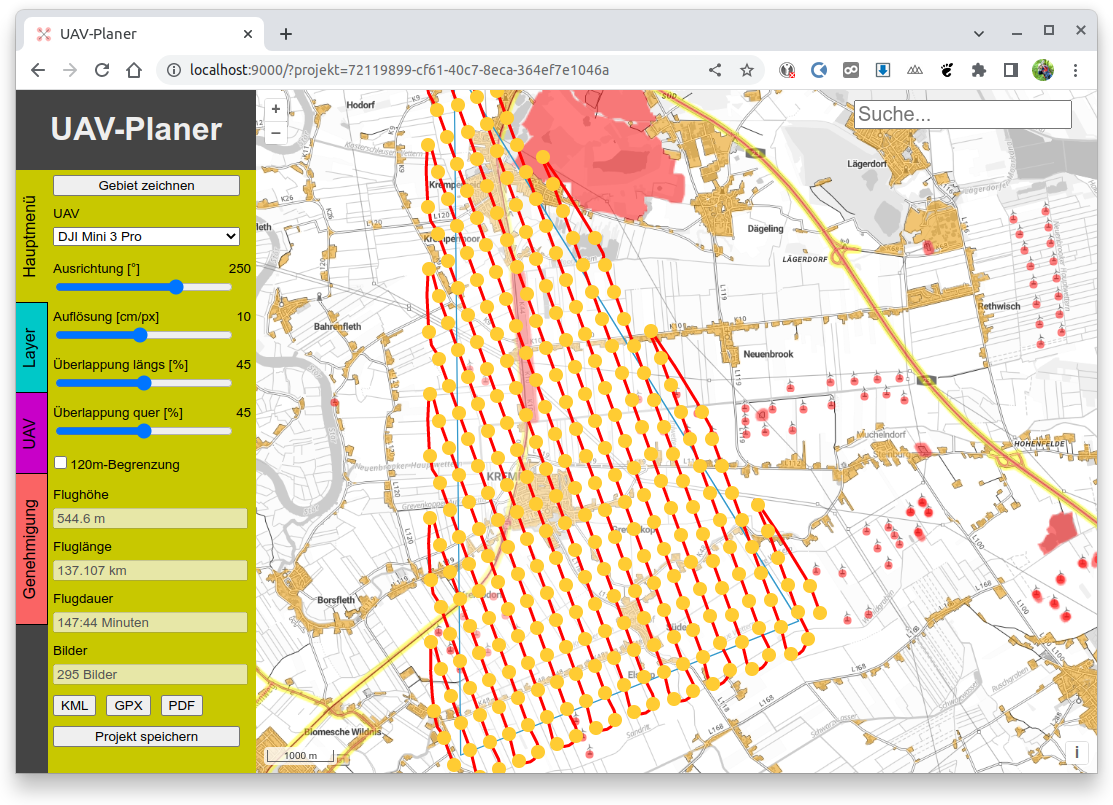
\includegraphics[width=1\textwidth]{./img/screenshot.png}
\centering
 \caption{Startbildschirm der Anwendung} %Bildunterschrift
 \label{img:screenshot} %ID fürs Bild
\end{figure}

\subsection{Auswählen des Messgebiet}
Die Navigation zum gewüsnchten Gebiet ist möglich mittels Verschieben der Karten Karten und zoomen sowie mit der Ortssuche oben rechts. Die Ortssuche bevorzugt dabei Orte, welche sich im oder Nahe des Kartenausschnittes befinden.

Anschließend kann nach einem Klick auf \textit{Gebiet zeichnen} in der Karte ein Polygon gezeichnet werden. Mit der linken Maustaste können neue Punkte gesetzt werden, mit der rechten Maustaste kann das Zeichnen abgeschlossen werden. Gegebenenfalls können die Stützpunkte des Polygones noch im Nachhinein verschoben werden.

\subsection{Einstellen der Parameter}
Es können nun die Parameter konfiguriert werden. Dazu bietet die Seitenleiste am linken Bildschirmrand verschiedene Optionen. Im Auswahlfeld ganz oben kann das zu nutzende UAV ausgewählt werden. Die Parameter für die einzelnen UAVs können im Reiter \textit{UAV} (siehe \autoref{uav}) verändert werden.

Mit dem Schieberegler \textit{Ausrichtung} kann die Flugrichtung bestimmt werden. Aktuell unterstützt die Planungssoftware nur das Muster einer Schlangenkurve. Mit dem nächsten Schieberegler \textit{Auflösung} kann die gewünschte Bodenauflösung festgelegt werden. Diese entscheidet damit dann bei gleichbleibender Kameraoptik über die mögliche Flughöhe und entsprechend die abgedeckte Fläche pro Bild.

Mit den beiden weiteren Schiebereglern \textit{Überlappung} kann die Überlappung der Bilder in Längs- und Querrichtung festgelegt werden. Diese entscheidet über die Anzahl der Bilder und die Dichte der einzelnen Flugbahnen.

Hieraus berechnet die Software dann die Trajektorie und die Positionen der einzlenen Bilder. Die sich hieraus ergebene Flughöhe und -länge, sowie die Anzahl der Bilder kann dem unteren Teil des Menüs entnommen werden.

\subsection{Speichern des Projektes / Datenexport}
Die Schaltflächen am unteren Rad des Hauptmenüs ermöglichen es, das Projekt zu speichern. Mit der Schaltfläche \textit{Projekt speichern} wird das Projekt in der Datenbank gesichert und ein Permalink erzeugt. Mit den Schaltflächen \textit{KML} und \textit{GPX} werden die Aufnahmepunkte im entsprechenden Format heruntergeladen und können beispielsweise in die Flugsteuerungssoftware des UAV importiert werden. Als weitere Möglichkeit kann der aktuelle Kartenauschnitt auch als PDF exportiert und beispielsweise ausgedruckt werden.

\subsection{Umschalten der Karte}
Der Reiter \textit{Layer} ermöglicht das Ändern der Hintergrundkarte und das Anzeigen von Fachdaten.

Von den Hintergrundkarten ist hierbei nur einer auswählbar, von den Fachdatenlayern sind auch mehrere auswählbar. Die \textit{Flugverbotszonen Hamburg} zeigen die Bereiche um die Flughäfen und -plätze, in denen ohne Sondergenehmigung kein Aufstieg erlaubt ist. Die \textit{Flugverbotszonen (BKG VectorTiles)} zeigen die Flugbeschränkungen, die sich aus der Örtlichkeit und der Luftverkehrsverordnung ergeben. Die \textit{Gebietsgrenzen} zeigen die Grenzen der einzelnen Landkreise und Bundesländer und damit die Zuständigkeiten an.

Alternativ ist es möglich, ein eigenes Bild als Kartenhintergrund, beispielsweise ein bereits erzeugtes Orthofoto, zu verwenden. Diese können mittels Drag-and-Drop als TIF-Datei eingebunden werden. Es reicht hierfür aus, eine GeoTIFF-Datei in EPSG:3857 auf die Karte zu ziehen. Das Bild wird dann entsprechend auf der Karte darstellt. Ein automatischer Zoom auf das Bild erfolgt aktuell noch nicht.

\subsection{UAV-Menü}
\label{uav}
Das \textit{UAV}-Menü ermöglicht das Hinzufügen und Ändern von UAV-Einstellungen. Diese werden dann in der Datenbank abgelegt.

Um einen Datensatz zu ändern, kann dieser in der Combobox oben ausgewählt werden und anschließend die Daten angepasst werden und entweder mit \textit{Ändern} direkt gespeichert oder mit \textit{Neu} als neuer Datensatz abgelegt werden. Um einen neuen Datensatz einzufügen, wird der passendste bestehende Datensatz ausgewählt und dann die Daten entsprechend verändert und dann mit \textit{Neu} der Datensatz gespeichert.

\subsection{Genehmigung-Menü}
Dieser Menü-Punkt ermöglicht das Prüfen des Projektgebietes auf genehmigungsfreies Fliegen. Hierbei werden die Beschränkungen aus der Luftverkehrsverordnung berück\-sichtigt, die sich auf die Örtlichkeit beziehen. Nicht geprüft wird aktuell der Abstand zu Flughäfen und -plätzen. Diese Regelungen werden vom Bundesland speziell für jedem Flughafen/-platz festgelegt und können daher nicht einfach so aus Geobasisdaten abgeleitet werden.

Nach dem Einzeichnen eines Projektgebietes kann mit dem \textit{Prüfen}-Button das aktuelle Gebiet geprüft werden. Sofern ein Eintrag in der Liste mit der Maus überfahren wird, leuchten die entsprechenden Gebiete rechts in der Karte auf. Aktuell wird hierbei die Bounding-Box überprüft, es kann also sein, dass zu viele Beschränkungen angezeigt werden. Außerdem wird nur mit Geometrien geprüft, die sich im Gebiet befinden. Von außerhalb reinragende Verbotszonen können daher noch nicht berücksichtigt werden.

\section{Technische Informationen}
\label{technische_information}

Das Benutzeroberfläche (Frontend) sowie die Schnittstelle zur Datenbank (Backend) basieren auf TypeScript, einen Aufsatz auf JavaScript, der JavaScript hauptsächlich um eine statische Typüberprüfung erweitert. Hierdurch wird die Identifikation von Fehlern in größeren Projekten erleichtert. \citep[S. 3]{typescript}

Außerdem wurde das gesamte FrontEnd objekt-orientiert programmiert. Das Klassendiagramm ist \autoref{img:klassendiagramm} zu sehen. Es wurde hierbei versucht, die Kopplung der einzelnen Klassen möglichst gering zu halten. Desweiteren wurde versucht, die Programmlogik, die Domänenklassen und die grafische Benutzeroberfläche in verschiedenene Klassen aufzuteilen, so dass Erweiterungen oder eine Umstrukturierung des Systemes möglich bleibt.

Das Backend ist in seinem Umfang relativ kompakt -- es besteht nur aus einer Datei -- so dass hier auf einen objekt-orientierten Ansatz verzichtet wurde.

\begin{figure} % setzt die Abbildung an genau diese Stelle, sonst landet sich oben auf der Seite
 \centering
 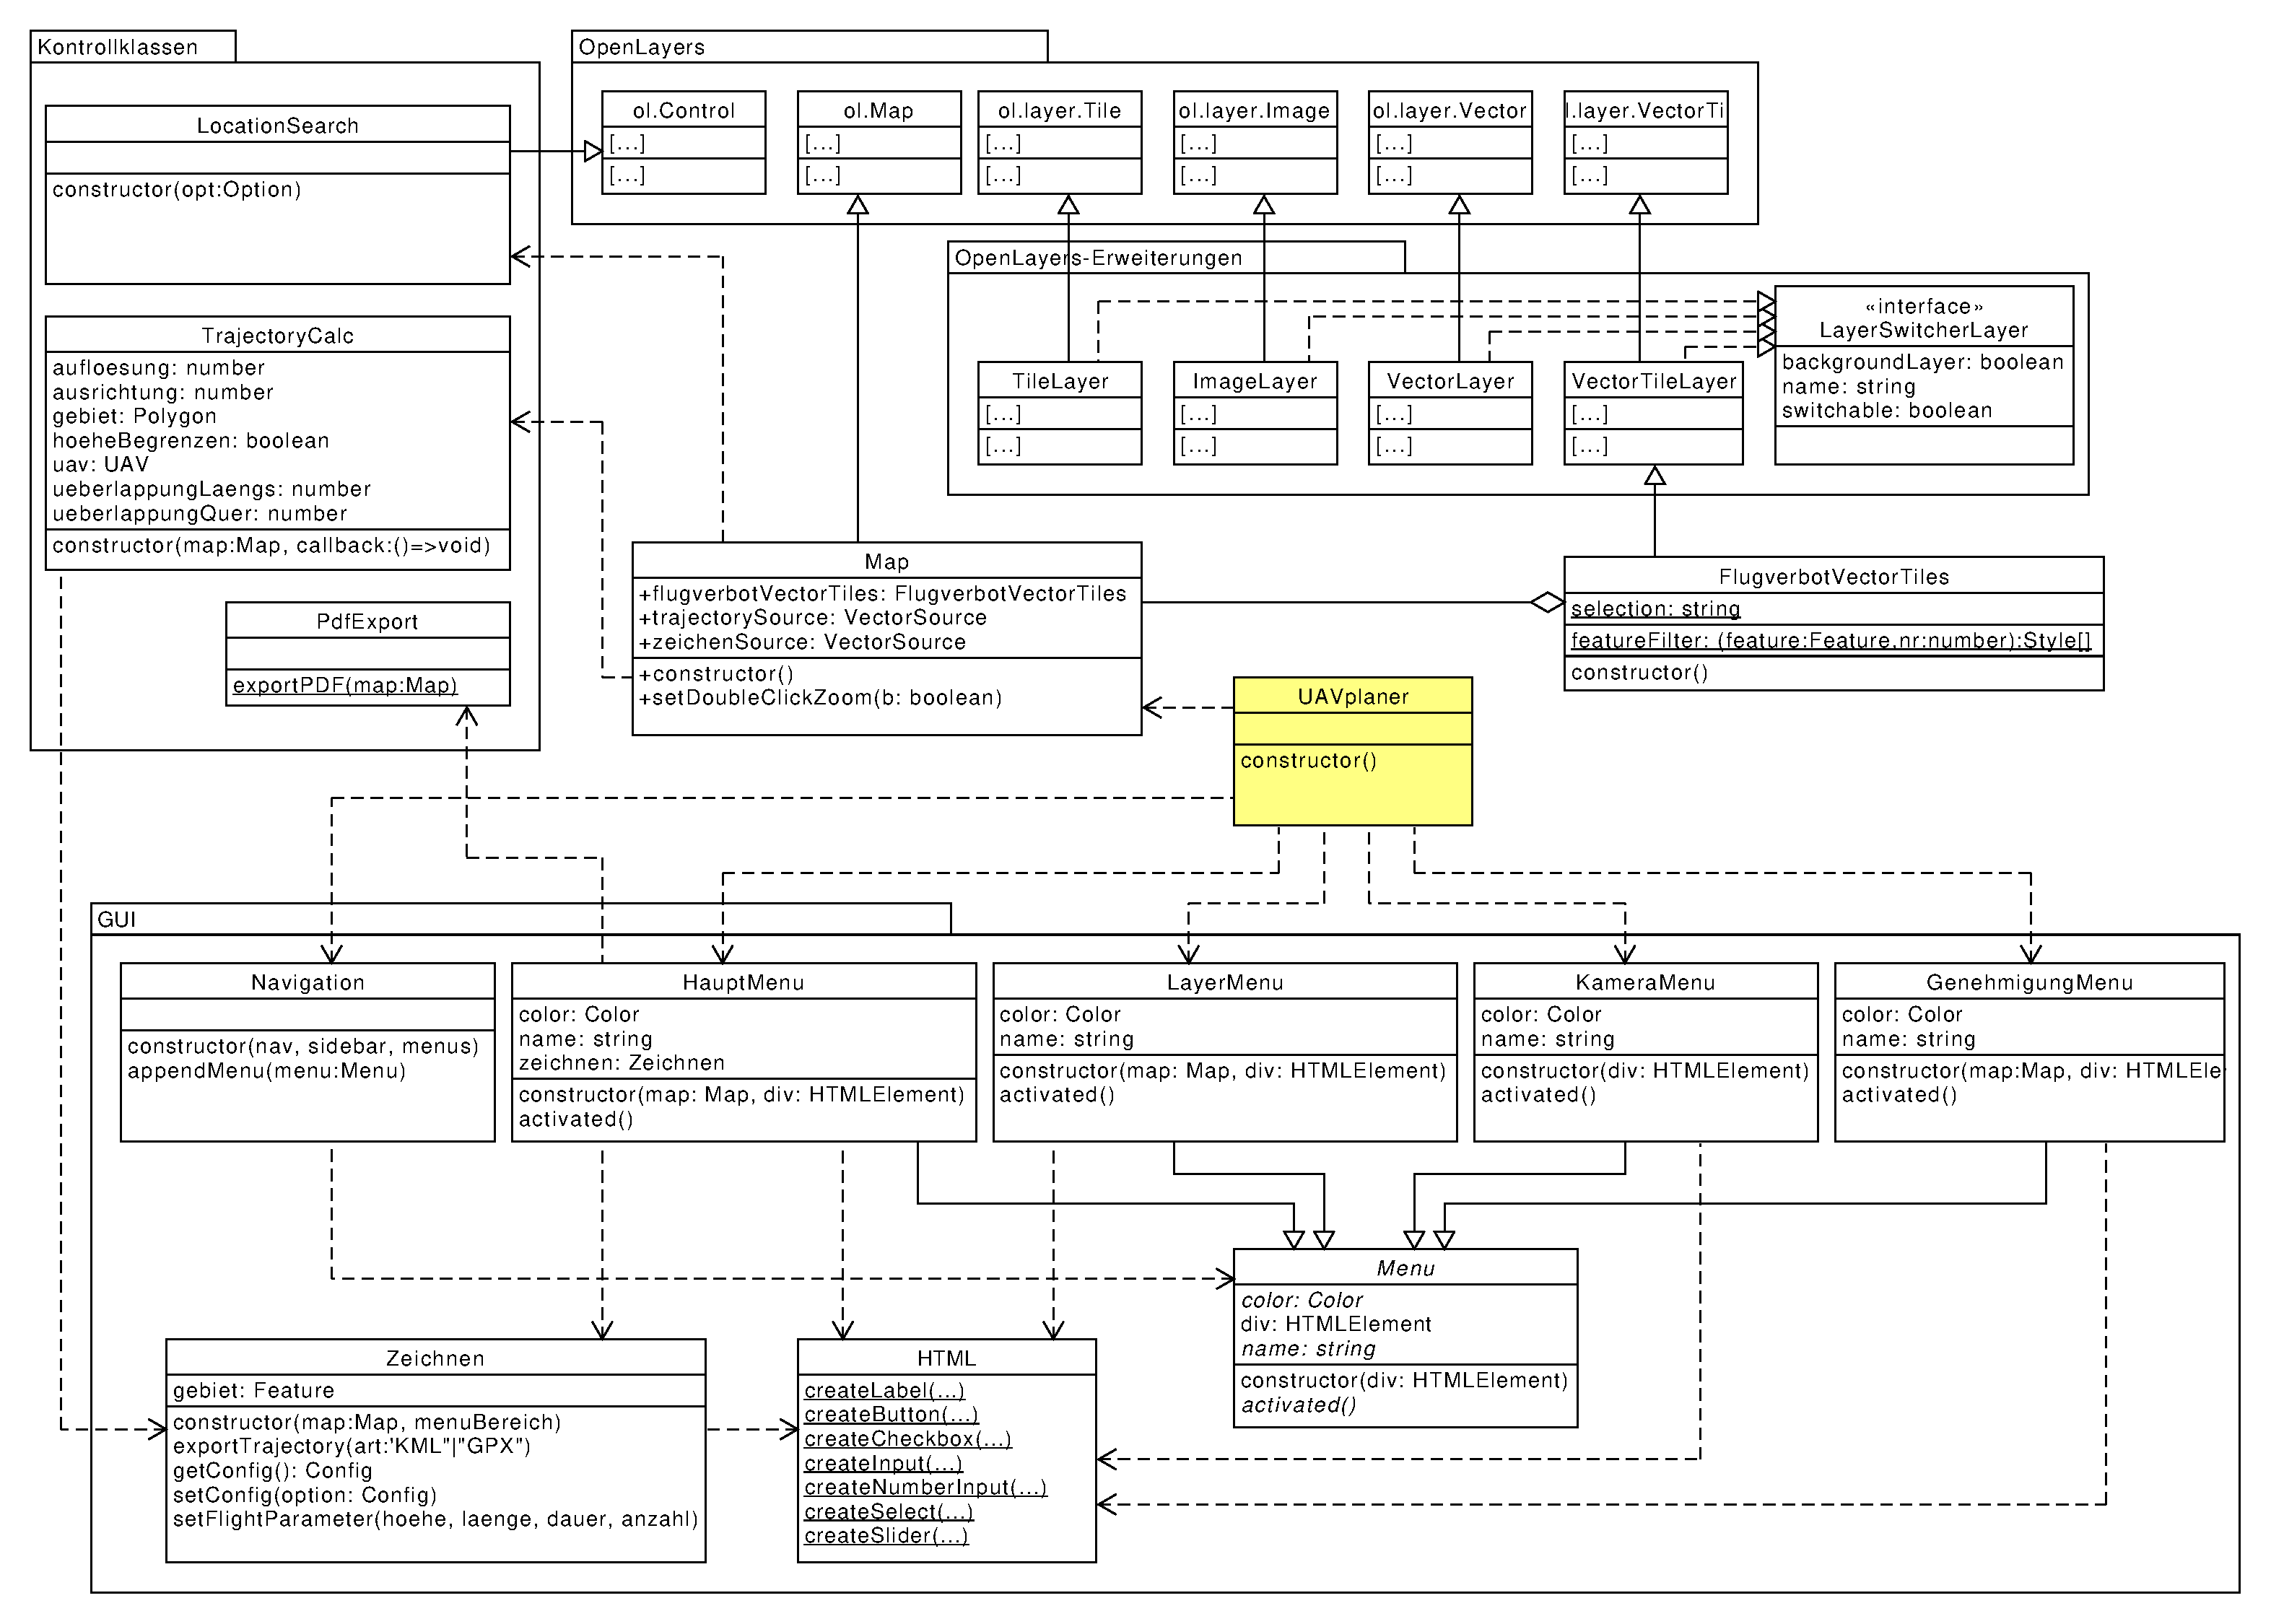
\includegraphics[width=1\textwidth]{./img/klassendiagramm.pdf}
\centering
 \caption{Klassendiagramm der Client-Anwendung} %Bildunterschrift
 \label{img:klassendiagramm} %ID fürs Bild
\end{figure}

Im Folgenden wird auf einzelne Komponenten detaillierter eingegangen.

\subsection{VectorTiles}
Für die Darstellung der Flugverbotsgebiete wurde der relativ neue Dienst Basemap des Bundesamtes für Kartographie und Geodäsie als VectorTiles genutzt. VectorTiles liefern ähnlich wie ein WFS Vectordaten aus, jedoch in gekachelter Form für den Zweck der Visualisierung. Vorteil gegenüber einem WMS ist, das hier das Darstellung der Daten selber festgelegt werden kann. Im Gegensatz zu einem WFS ist er aber auf die Darstellung und auf möglichst geringe Datenmengen optimiert.

Die Visualisierung wurde hier so angepasst, dass Beispielsweise Bundesstraßen entsprechend der Größe ihrer Flugbeschränkungen dargestellt werden. Der Reiter \textit{Genehmigung} nutzt diese Daten dann auch zur Prüfung auf Flugbeschränkungen und ermöglicht auch das Aufblinken der einzelnen Beschränkungen.

\subsection{Datenspeicherung/REST-Schnittstelle}
Die Speicherung der Projekte und der UAV-Modelle erfolgt in einer SQLite-Datenbank auf dem Server. So wird auch eine lokale Nutzung einfach möglich, da als Voraussetzung für den Server nur eine Node.js-Installation notwendig ist.

Die Kommunikation mit dem Server und erfolgt über eine REST-Schnittstelle.

\subsection{Bildflugberechnungen}
Die Bildflugplanung erfolgt aktuell nur in Form von Nadirbildern. Eine evtl. für die Berechnung der Kameraparameter optimalere Aufnahme \citep{opendronemap} \todo{Seitenzahl} von leicht geneigten Bildern ist aktuell nicht möglich. Die Berechnung der Bildgröße erfolgt vereinfacht mit dem Strahlensatz und der Annahme eines ebenen Grundes:

\begin{equation*}
    \frac{\text{[Brennweite]}}{\text{[Sensorbreite]}} =  \frac{\text{[Flughöhe]}}{\text{[Bildbreite]}} 
\end{equation*}

Eine Erweiterung um die Berücksichtigung des Geländes erscheint als relativ aufwendig und wurde daher verworfen.

\subsection{Responsible-Design}
Der UAV-Planer ist so gestaltet, dass er sich auch an kleine Display wie Tablets oder Mobiltelefone anpasst. Hierdurch wird auch eine mobile Nutzung ermöglicht.

\clearpage
%Literatur
\renewcommand\UrlFont\itshape
\renewcommand{\refname}{Literaturverzeichnis}
\bibliography{webgis}
%\printbibliography
\listoffigures
%\listoftables
%\lstlistoflistings

\end{document}